\documentclass{article}

\usepackage{amsmath,amssymb}
\usepackage{tikz}
\usepackage{pgfplots}
\usepackage{xcolor}
\usepackage[left=2.1cm,right=3.1cm,bottom=3cm,footskip=0.75cm,headsep=0.5cm]{geometry}
\usepackage{enumerate}
\usepackage{enumitem}
\usepackage{marvosym}
\usepackage{tabularx}
\usepackage[amsmath,thmmarks,standard]{ntheorem}
\usepackage{mathtools}

\usepackage[utf8]{inputenc}

\renewcommand*{\arraystretch}{1.4}
\newcommand{\E}{\mathbb{E}}

\newcolumntype{L}[1]{>{\raggedright\arraybackslash}p{#1}}
\newcolumntype{R}[1]{>{\raggedleft\arraybackslash}p{#1}}
\newcolumntype{C}[1]{>{\centering\let\newline\\\arraybackslash\hspace{0pt}}m{#1}}

\DeclareMathOperator{\tr}{tr}
\DeclareMathOperator{\Var}{Var}
\DeclareMathOperator{\Cov}{Cov}
\renewcommand{\E}{\mathbb{E}}

\newtheorem{thm}{Theorem}
\newtheorem{lem}{Lemma}

\title{\textbf{Einführung in die Produktion, Tutorium 5}}
\author{\textsc{Henry Haustein}}
\date{}

\begin{document}
	\maketitle
	
	\section*{Aufgabe 10}
	\begin{enumerate}[label=(\alph*)]
		\item Definitionen aus der Vorlesung
		\begin{itemize}
			\item Bruttoprimärbedarf: Gesamtheit der verkaufsbestimmten Mengen an Endprodukten, Halbfertigerzeugnissen und Verbrauchsmaterial
			\item Nettoprimärbedarf: Subtraktion der Lagerbestände vom Bruttoprimärbedarf
			\item Sekundärbedarf: Materialien, die zur Bereitstellung bzw. Produktion des Nettoprimärbedarfs benötigt werden
			\item Tertiärbedarf: Hilfs- und Betriebsstoffe, die nicht eindeutig einem Produkt zugeordnet werden können.
		\end{itemize}
		\item Graph
		\begin{center}
			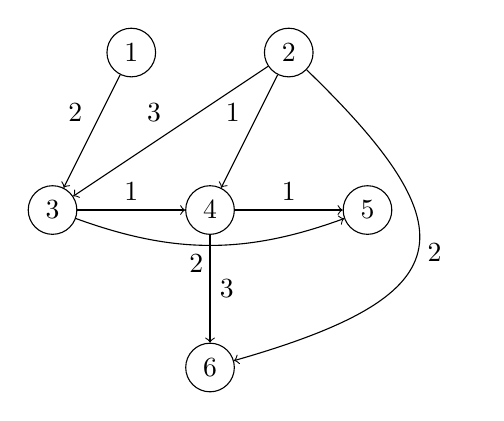
\begin{tikzpicture}
			\node[circle,draw=black, fill=white] (1) at (0,0) {1};
			\node[circle,draw=black, fill=white] (2) at (2,0) {2};
			\node[circle,draw=black, fill=white] (3) at (-1,-2) {3};
			\node[circle,draw=black, fill=white] (4) at (1,-2) {4};
			\node[circle,draw=black, fill=white] (5) at (3,-2) {5};
			\node[circle,draw=black, fill=white] (6) at (1,-4) {6};
			
			\draw[->] (1) to node[above left] {2} (3);
			\draw[->] (2) to node[above left] {3} (3);
			\draw[->] (2) to node[above left] {1} (4);
			\draw[->] (2) to[bend left=60,looseness=2] node[right] {2} (6);
			\draw[->] (3) to node[above] {1} (4);
			\draw[->] (3) to[bend right=20] node[below,xshift=-5] {2} (5);
			\draw[->] (4) to node[above] {1} (5);
			\draw[->] (4) to node[right] {3} (6);
			\end{tikzpicture}
		\end{center}
		\item Negativer Nettoprimärbedarf stellt vorhandene Produkte im Lager dar.
		\item Gozintolistenverfahren
		\begin{center}
			\begin{tabular}{c|cc|cc|cc|cc}
				& $v_1$ & $N_1$ & $v_2$ & $N_2$ & $v_3$ & $N_3$ & $v_4$ & $N_4$ \\
				\hline
				1 & 1 & 0 & 1 & 0 & 1 & 0 & 0 & 400 \\
				2 & 3 & 0 & 2 & 400 & 2 & 400 & 0 & 400 + 600 \\
				3 & 2 & 0 & 2 & 0 & 1 & 200 & 0 & \\
				4 & 2 & -800 & 1 & -800 + 600 & 0 & -800 + 600 + 100 & 0 & -800 + 600 + 100 \\
				5 & 0 & 100 & 0 & 100 & 0 & & 0 & \\
				6 & 0 & 200 & 0 & & 0 & & 0 &
			\end{tabular}
		\end{center}
		\item $R^T=(400,1000,200,-100,100,200)$
	\end{enumerate}

	\section*{Aufgabe 11}
	\begin{enumerate}[label=(\alph*)]
		\item ei einer Mengenübersichtsstückliste sind die Mengen von alles Ausgangs- und Zwischenprodukten für 1 Endprodukt angegeben. Bei mehrstufigen Prozessen müssen diese Zahlen kumuliert werden.
		\item Mengenübersichtsstückliste für das Produkt $P$
		\begin{center}
			\begin{tabular}{c|c|c}
				\textbf{Sachnummer} & \textbf{Menge} & \textbf{Bezeichnung} \\
				\hline
				$E$ & 22 + 12 = 34 & Einsatzfaktor \\
				$Z_1$ & 2 + 1 + 8 = 11 & Zwischenprodukt 1 \\
				$Z_2$ & 4 & Zwischenprodukt 2 \\
				$Z_3$ & 1 & Zwischenprodukt 3
			\end{tabular}
		\end{center}
		\item Gozintoliste
		\begin{center}
			\begin{tabular}{c|c|c}
				Eingangsknoten $i$ & Ausgangsknoten $j$ & Bewertung $d_{ij}$ \\
				\hline
				2 & 1 & 2 \\
				3 & 1 & 3 \\
				3 & 2 & 2 \\
				4 & 2 & 1 \\
				5 & 2 & 2 \\
				4 & 3 & 4 \\
				5 & 4 & 1
			\end{tabular}
		\end{center}
		\item Gozintolistenverfahren
		\begin{center}
			\begin{tabular}{c|cc|cc|cc|cc}
				& $v_1$ & $N_1$ & $v_2$ & $N_2$ & $v_3$ & $N_3$ & $v_4$ & $N_4$ \\
				\hline
				$E$ & 2 & 0 & 2 & 0 & 2 & 0 & 0 & 500 \\
				$Z_1$ & 3 & 0 & 2 & 100 & 1 & 100 + 150 & 0 & \\
				$Z_2$ & 1 & -700 & 1 & -700 & 0 & -700 + 600 & 0 & -100 \\
				$Z_3$ & 1 & 100 & 0 & 100 + 50 & 0 & & 0 & \\
				$P$ & 0 & 50 & 0 & & 0 & & 0 & \\
			\end{tabular}
		\end{center}
		\item $R^T=(500,250,-100,150,50)$
		\item Da wir noch 100 Einheiten von $Z_2$ auf dem Lager haben, könnte der Lagerbestand von $Z_2$ auch um diese sinken, ohne unsere Kalkulation zu zerstören.
	\end{enumerate}
	
\end{document}